%!TEX ROOT=formularioMatematica.tex

\section{Calcolo approssimato}
Il calcolo approssimato si occupa di approssimare il valore di una funzione o di un integrale. Oltre
alle ovvie utilità, diventa anche molto comodo quando non si conoscono le primitive dell'integrale
oppure la soluzione di un'equazione non è risolvibile algebricamente. Tutti i metodi si bastano sul
\textbf{teorema degli zeri}. C'è una necessità però, che lo zero nell'intervallo sia unico. Ovvero
\begin{equation*}
  \exists!\,c\in]a,b[\suchthat f(c)=0\quad\text{se}\quad f(a)\cdot f(b) < 0
\end{equation*}
Questo è assicurato dalle seguenti condizioni
\begin{equation*}
  f'(x)>0\lor f'(x)<0\quad\forall x\in]a,b[
\end{equation*}
o
\begin{equation*}
  f''(x)>0\lor f''(x)<0\quad\forall x\in]a,b[
\end{equation*}

\subsection{Approssimazione numerica}
Questi metodi seguenti sono utili ad approssimare una funzione o la soluzione di un'equazione.

\subsubsection{Metodo di bisezione}
Anche detto metodo di dicotomia è forse il più facile da ricordare ma il più lento a convergere.\\
Esso si basa sul Teorema degli zeri e la sua ipotesi.
\begin{center}
  \begin{tikzpicture}
    \begin{axis}[xmin=-1,ymin=-2,xmax=5,ymax=3]
      \addplot[thick,red,smooth,samples=500,domain=0.01:4] {-ln(x/pi)-1}; 
      \draw[thick,dashed] (0.5,-1.5) -- (0.5,0.8378);
      \draw[thick,dashed] (1.75,-1.5) -- (1.75,-0.4148);
      \draw[thick,dashed] (4,-1.5) -- (4,-1.2415);
      \draw[thick,dashed] (1.125,-1.5) -- (1.125,0.0269);

      \draw[thick,blue] (0.5,-1.5) -- (4,-1.5);
      \draw[thick,blue] (1.125,-1.3) -- (1.75,-1.3);
    \end{axis}
  \end{tikzpicture}
\end{center}
Come si evice dal disegno si prendono gli estremi e si trova il punto medio $x_0$. A quel punto
si trova il segno del prodotto degli estremi per il punto medio. Si sceglie l'estremo che ha segno
negativo (e che quindi contiene la soluzione cercata). Si calcola il nuovo punto medio e si va
avanti fino a che non si raggiunge la precisione desiderata.

\subsubsection{Metodo delle tangenti}
\begin{center}
  \begin{tikzpicture}
    \begin{axis}[
      xmin=0,ymin=-1,xmax=4,ymax=4,
      tangent/.style={%
        add node at x={#1}{%
          [
          sloped,
          append after command={(\tikzlastnode.west) edge [thick, blue] (\tikzlastnode.east)},
          minimum width=5cm
          ]
        },
      },
      ]
      \addplot[thick,draw=red,smooth,samples=500,domain=0.01:4,tangent=0.5] {-ln(x/pi)};
      \addplot[thick,draw=red,smooth,samples=500,domain=0.01:4,tangent=1.5] {-ln(x/pi)};
      \addplot[thick,draw=red,smooth,samples=500,domain=0.01:4,tangent=2.3] {-ln(x/pi)};
      \draw[thick,dashed] (0.5,1.8378) -- (0.5,0) node[pos=1,below]{$x_0$};
      \draw[thick,dashed] (1.5,0.7392) -- (1.5,0) node[pos=1,below]{$x_1$};
      \draw[thick,dashed] (2.3,0.3111) -- (2.3,0) node[pos=1,below]{$x_2$};
    \end{axis}
  \end{tikzpicture}
\end{center}
Da questo disegno possiamo capire il procedimento che sta alla base di questo metodo. 
Il primo punto analizzato è $x_0=a$, presa la tangente in quel punto possiamo vedere che il punto 
di intersezione con l'asse delle $x$ è una pessima approsimazione dello zero della funzione. 
Il punto $x_1$ invece è un'approssimazione migliore e così via. Infatti questo è un metodo 
iterativo la cui formula generale è
\begin{equation*}
  \begin{cases}
    x_n=x_{n-1}-\frac{f(x_{n-1})}{f'(x_{n-1})}\\
    \begin{cases}
      x_0=a, & f(x_0)\cdot f''(x) > 0\\
      x_0=b, & f(x_0)\cdot f''(x) < 0
    \end{cases}
  \end{cases}
\end{equation*}

\subsubsection{Metodo delle secanti}
\begin{center}
  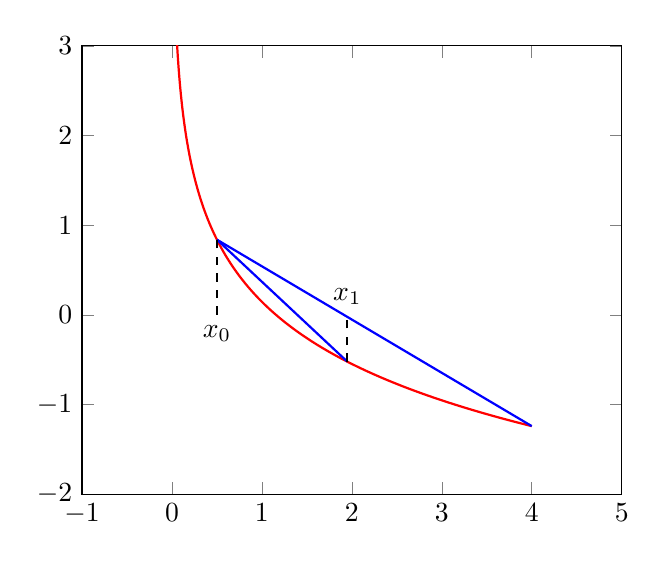
\begin{tikzpicture}
    \begin{axis}[xmin=-1,ymin=-2,xmax=5,ymax=3]
      \addplot[thick,red,smooth,samples=500,domain=0.01:4] {-ln(x/pi)-1}; 
      \draw[thick,blue] (0.5,0.8378) -- (4,-1.2415);
      \draw[thick,blue] (0.5,0.8378) -- (1.95,-0.5230);

      \draw[thick,dashed] (0.5,0) -- (0.5,0.8378) node[pos=0,below]{$x_0$};
      \draw[thick,dashed] (1.95,-0.5230) -- (1.95,0) node[pos=1,above]{$x_1$};
    \end{axis}
  \end{tikzpicture}
\end{center}
Il disegno permette di comprendere il sistema che sta alla base di questo metodo. Si scegla $a$ o 
$b$ come punto cardine e si trovino le secanti alla funzione tra $a$ e $x_n$ o $b$ e $x_n$. Il
punto di intersezione della secante con l'asse delle $x$ sarà via via un'approssimazione migliore.
Anche questo metodo è iterativo con formula generale
\begin{equation*}
  \begin{cases}
    x_n=x_{n-1} - \frac{f(l)(x_{n-1}-l)}{f(x_{n-1}-f(l))}\\
    \begin{cases}
      x_0=a\land l=b, & f(x_0)\cdot f''(x) < 0\\
      x_0=b\land l=a, & f(x_0)\cdot f''(x) > 0
    \end{cases}
  \end{cases}
\end{equation*}

\subsection{Integrazione numerica}
Di seguito saranno riportati metodi per approssimare l'integrale definito di una funzione.

\subsubsection{Metodo dei rettangoli}
\begin{center}
  \begin{tikzpicture}
    \begin{axis}[xmin=0,ymin=0,xmax=7,ymax=7]
      \addplot[blue,thick,domain=1:6,samples=50,smooth] {sin(deg(x-2))*(x-5)+3};
      \addplot[fill=yellow,fill opacity=0.5,integral=1:6,integral segments=10] 
        {sin(deg(x-2))*(x-5)+3};
    \end{axis}
  \end{tikzpicture}
\end{center}
Il metodo dei rettangoli va atrovare l'area di rettangoli di base $f(x)$ e altezza $h$. Una 
maggiore quantità di questi rettangoli porta ad una maggiore precisione. Infatti andando a prendere
il limite si ottiene la definizione di integrale definito.
\begin{equation*}
  \int\limits_{a}^{b} f(x)\dif x \approx \sum\limits^{n}_{i=0} f(a+ih)h = \sum\limits^{n}_{i=1} f(x_i)
  \frac{b-a}{n}
\end{equation*}
Questa formula va usata se si vuole prendere come ultimo rettangolo quello più a destra. La 
seguente invece va usata se si vuole partire dal primo rettangolo più a sinistra
\begin{equation*}
  \int\limits_{a}^{b} f(x)\dif x \approx \sum\limits^{n-1}_{i=1} f(a+ih)h = \sum\limits^{n-1}_{i=0} 
  f(x_i)\frac{b-a}{n}
\end{equation*}

\subsubsection{Metodo dei trapezi}
\begin{center}
  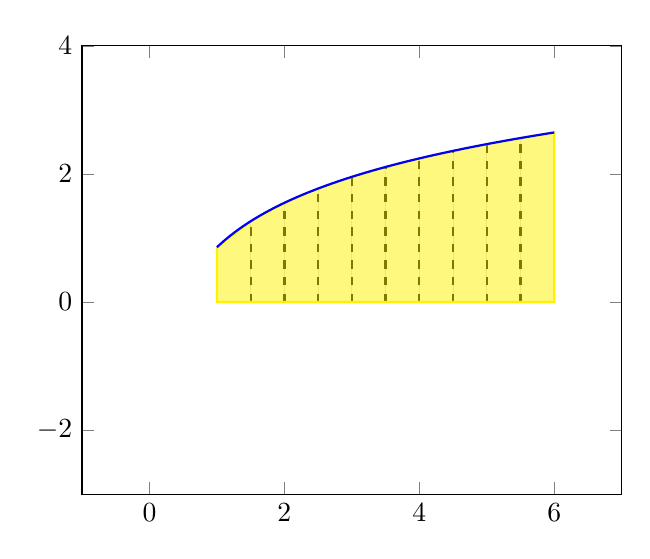
\begin{tikzpicture}
    \begin{axis}[xmin=-1,ymin=-3,xmax=7,ymax=4]
      \filldraw[thick,dashed]
        (1,0) -- (1,0.8552)
        (1.5,0) -- (1.5,1.2607)
        (2,0) -- (2,1.5484)
        (2.5,0) -- (2.5,1.7715)
        (3,0) -- (3,1.9538)
        (3.5,0) -- (3.5,2.1080)
        (4,0) -- (4,2.2415)
        (4.5,0) -- (4.5,2.3593)
        (5,0) -- (5,2.4647)
        (5.5,0) -- (5.5,2.5600)
        (6,0) -- (6,2.6470);
      \filldraw[thick, yellow, fill opacity=0.5] (1,0) --
        (1,0.8552) -- (1.5,1.2607) -- (2,1.5484) -- (2.5,1.7715) -- (3,1.9538) -- (3.5,2.1080) --
        (4,2.2415) -- (4.5,2.3593) -- (5,2.4647) -- (5.5,2.5600) -- (6,2.6470) -- (6,0) -- cycle;
      \addplot[blue,thick,domain=1:6,samples=50,smooth] {ln(x/pi)+2};
    \end{axis}
  \end{tikzpicture}
\end{center}
Il metodo dei trapezi invece di prendere dei triangoli, prende dei trapezi in cui uno dei lati è
il segmento che va  tra due punti della funzione. L'approssimazione diventa quindi
\begin{equation*}
  \int\limits_{a}^{b} f(x)\dif x = \frac{b-a}{n}\left[ \frac{f(x_0)+f(x_n)}{2}+
  \sum\limits^{n-1}_{i=1} f(x_i) \right]
\end{equation*}
